%! Author = ben
%! Date = 24.10.2023

\documentclass[./entry.tex]{subfiles}

\begin{document}
    \chapter{Integration in den Unterricht}

    Im Unterricht können Sortieralgorithmen auf verschiedene Arten den Schülern näher gebracht werden.
    Die einfachste Möglichkeit ist die visuelle Darstellung der Algorithmen.
    Hierbei bekommt jeder Schüler ein Blatt Papier, auf dem eine Zahl abgebildet ist.
    Jede Zahl sollte, wenn möglich, nur einmal verwendet werden, damit eine eindeutige Sortierung erkennbar ist.
    Die Schüler stellen sich nun in einer Reihe auf, die zu Anfang unsortiert ist.
    Anschließend wird der gewählte Algorithmus schrittweise durchgeführt.
    Es ist zu empfehlen, mit einem einfachen Algorithmus, wie dem \dq Bubble-Sort\dq-Verfahren zu beginnen,
    damit das Prinzip verstanden werden kann.

    \paragraph{Beispiel}
    Es wurden die Zahlen eins bis vier unter den Schülern aufgeteilt, welche sich in eine
    unsortierte Reihefolge aufgestellt haben und anschließend das \dq Bubble-Sort\dq-Verfahren
    durchführen. Folgende Abbildung zeigt die Ausgangssituation.
    \vspace{0.5cm}

    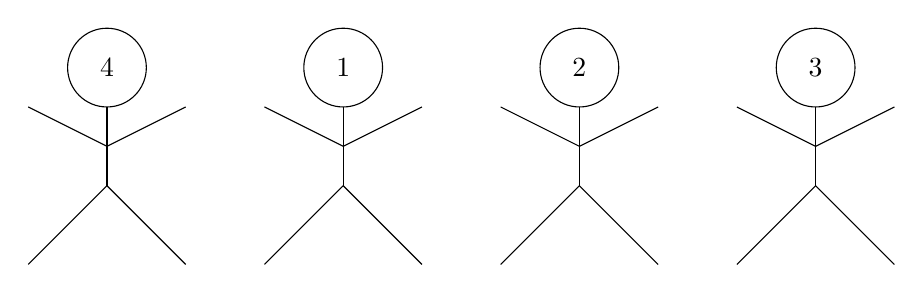
\begin{tikzpicture}
        %% PERSON (4)
        % Head
        \draw (2,2) circle (0.5cm) node {4};
        % Body
        \draw (2,1.5) -- (2,0.5);
        % Legs
        \draw (2,0.5) -- (1,-0.5);
        \draw (2,0.5) -- (3,-0.5);
        % Arms
        \draw (2,1) -- (1,1.5);
        \draw (2,1) -- (3,1.5);

        %% PERSON (1)
        \draw (5,2) circle (0.5cm) node {1};
        % Body
        \draw (5,1.5) -- (5,0.5);
        % Legs
        \draw (5,0.5) -- (4,-0.5);
        \draw (5,0.5) -- (6,-0.5);
        % Arms
        \draw (5,1) -- (4,1.5);
        \draw (5,1) -- (6,1.5);

        %% PERSON (2)
        \draw (8,2) circle (0.5cm) node {2};
        % Body
        \draw (8,1.5) -- (8,0.5);
        % Legs
        \draw (8,0.5) -- (7,-0.5);
        \draw (8,0.5) -- (9,-0.5);
        % Arms
        \draw (8,1) -- (7,1.5);
        \draw (8,1) -- (9,1.5);

        %% PERSON (3)
        \draw (11,2) circle (0.5cm) node {3};
        % Body
        \draw (11,1.5) -- (11,0.5);
        % Legs
        \draw (11,0.5) -- (10,-0.5);
        \draw (11,0.5) -- (12,-0.5);
        % Arms
        \draw (11,1) -- (10,1.5);
        \draw (11,1) -- (12,1.5);
    \end{tikzpicture}


    Nun wird der Algorithmus schrittweise durchgeführt.
    In der folgenden Grafik ist der erste Schritt dargestellt.
    Die Schüler vergleichen die erste und zweite Zahl.
    Da die erste Zahl größer ist, werden die beiden Zahlen getauscht.
    \vspace{0.5cm}

    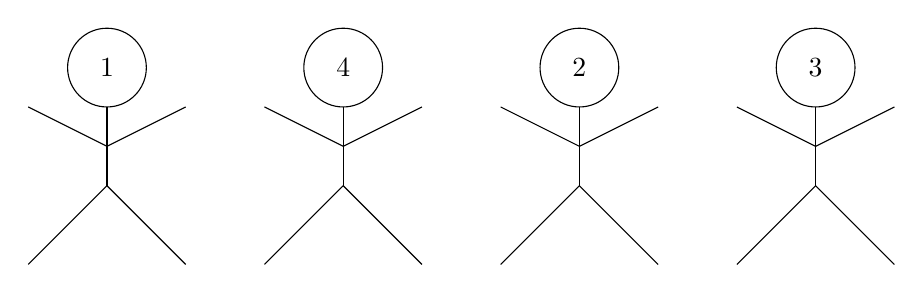
\begin{tikzpicture}
        % Head
        \draw (2,2) circle (0.5cm) node {1};
        % Body
        \draw (2,1.5) -- (2,0.5);
        % Legs
        \draw (2,0.5) -- (1,-0.5);
        \draw (2,0.5) -- (3,-0.5);
        % Arms
        \draw (2,1) -- (1,1.5);
        \draw (2,1) -- (3,1.5);

        \draw (5,2) circle (0.5cm) node {4};
        % Body
        \draw (5,1.5) -- (5,0.5);
        % Legs
        \draw (5,0.5) -- (4,-0.5);
        \draw (5,0.5) -- (6,-0.5);
        % Arms
        \draw (5,1) -- (4,1.5);
        \draw (5,1) -- (6,1.5);

        \draw (8,2) circle (0.5cm) node {2};
        % Body
        \draw (8,1.5) -- (8,0.5);
        % Legs
        \draw (8,0.5) -- (7,-0.5);
        \draw (8,0.5) -- (9,-0.5);
        % Arms
        \draw (8,1) -- (7,1.5);
        \draw (8,1) -- (9,1.5);

        \draw (11,2) circle (0.5cm) node {3};
        % Body
        \draw (11,1.5) -- (11,0.5);
        % Legs
        \draw (11,0.5) -- (10,-0.5);
        \draw (11,0.5) -- (12,-0.5);
        % Arms
        \draw (11,1) -- (10,1.5);
        \draw (11,1) -- (12,1.5);
    \end{tikzpicture}

    Anschließend werden die zweite und dritte Zahl verglichen.
    Da die zweite Zahl größer ist, werden die beiden Zahlen getauscht.
    \vspace{0.5cm}

    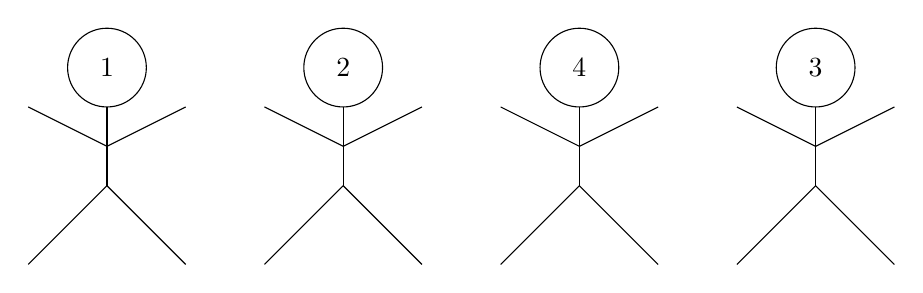
\begin{tikzpicture}
        % Head
        \draw (2,2) circle (0.5cm) node {1};
        % Body
        \draw (2,1.5) -- (2,0.5);
        % Legs
        \draw (2,0.5) -- (1,-0.5);
        \draw (2,0.5) -- (3,-0.5);
        % Arms
        \draw (2,1) -- (1,1.5);
        \draw (2,1) -- (3,1.5);

        \draw (5,2) circle (0.5cm) node {2};
        % Body
        \draw (5,1.5) -- (5,0.5);
        % Legs
        \draw (5,0.5) -- (4,-0.5);
        \draw (5,0.5) -- (6,-0.5);
        % Arms
        \draw (5,1) -- (4,1.5);
        \draw (5,1) -- (6,1.5);

        \draw (8,2) circle (0.5cm) node {4};
        % Body
        \draw (8,1.5) -- (8,0.5);
        % Legs
        \draw (8,0.5) -- (7,-0.5);
        \draw (8,0.5) -- (9,-0.5);
        % Arms
        \draw (8,1) -- (7,1.5);
        \draw (8,1) -- (9,1.5);

        \draw (11,2) circle (0.5cm) node {3};
        % Body
        \draw (11,1.5) -- (11,0.5);
        % Legs
        \draw (11,0.5) -- (10,-0.5);
        \draw (11,0.5) -- (12,-0.5);
        % Arms
        \draw (11,1) -- (10,1.5);
        \draw (11,1) -- (12,1.5);
    \end{tikzpicture}

    Abschließend werden die dritte und vierte Zahl verglichen.
    Da die dritte Zahl größer ist, werden die beiden Zahlen getauscht.

    \vspace{0.5cm}

    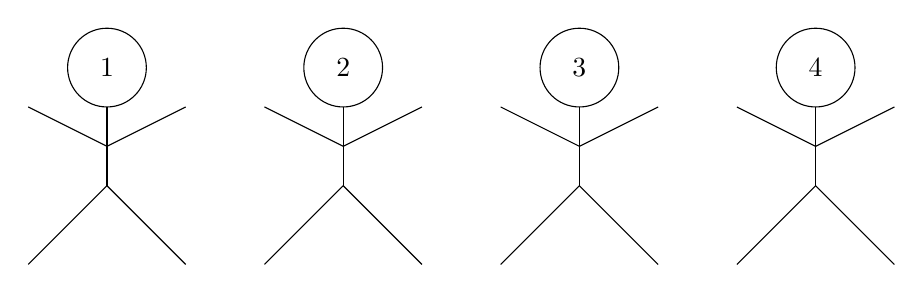
\begin{tikzpicture}
        % Head
        \draw (2,2) circle (0.5cm) node {1};
        % Body
        \draw (2,1.5) -- (2,0.5);
        % Legs
        \draw (2,0.5) -- (1,-0.5);
        \draw (2,0.5) -- (3,-0.5);
        % Arms
        \draw (2,1) -- (1,1.5);
        \draw (2,1) -- (3,1.5);

        \draw (5,2) circle (0.5cm) node {2};
        % Body
        \draw (5,1.5) -- (5,0.5);
        % Legs
        \draw (5,0.5) -- (4,-0.5);
        \draw (5,0.5) -- (6,-0.5);
        % Arms
        \draw (5,1) -- (4,1.5);
        \draw (5,1) -- (6,1.5);

        \draw (8,2) circle (0.5cm) node {3};
        % Body
        \draw (8,1.5) -- (8,0.5);
        % Legs
        \draw (8,0.5) -- (7,-0.5);
        \draw (8,0.5) -- (9,-0.5);
        % Arms
        \draw (8,1) -- (7,1.5);
        \draw (8,1) -- (9,1.5);

        \draw (11,2) circle (0.5cm) node {4};
        % Body
        \draw (11,1.5) -- (11,0.5);
        % Legs
        \draw (11,0.5) -- (10,-0.5);
        \draw (11,0.5) -- (12,-0.5);
        % Arms
        \draw (11,1) -- (10,1.5);
        \draw (11,1) -- (12,1.5);
    \end{tikzpicture}

    Jetzt ist die Reihefolge sortiert und die Prozedur kann
    mit einer neuen Reihenfolge oder einem anderen Algorithmus wiederholt werden.

\end{document}